\documentclass[12pt,a4paper]{article}
\usepackage[polish]{babel}
\usepackage[T1]{fontenc}
\usepackage[utf8x]{inputenc}
\usepackage{hyperref}
\usepackage{url}
\usepackage{graphicx}
\usepackage{float}

\addtolength{\hoffset}{-1.5cm}
\addtolength{\marginparwidth}{-1.5cm}
\addtolength{\textwidth}{3cm}
\addtolength{\voffset}{-1cm}
\addtolength{\textheight}{2.5cm}
\setlength{\topmargin}{0cm}
\setlength{\headheight}{0cm}

\begin{document}

\title{Bazy Danych\\Projekt Karta Pacjenta}
\date{\today}

\maketitle

\tableofcontents
\clearpage

% zad 1
\section{Autorzy}
\begin{center}
   \large
{Krzysztof Czarnecki

Błażej Czekała


Patryk Wenz

Hubert Braun} 
\end{center}

\section{Opis projektu}
Generowanie raportu z badania dla pacjenta (format PDF, ODT, DOC, lub inny).


\section{Wybrane technologie}
\section{Wybrane technologie}
\begin{itemize}
    \item Spring Boot
    \item Spring Security
    \item PostgreSQL
    \item Java
    \item Angular
\end{itemize}


\section{Zadania}
\begin{enumerate}
    \item Napisanie serwera.
    \item Dodanie zabezpieczeń użytkownika.
    \item Anonimizacja danych w bazie.
    \item Testy obciążeniowe.
\end{enumerate}

\subsection{Kontrola wersji}
Do pracy zespołowej wykorzystaliśmy znane i lubiane narzędzie \textit{GitHub}. Umożliwiło nam to sprawne dzielenie się zmianami w kodzie, zarządzanie i wersjonowanie go.

\subsection{Baza danych}
\begin{figure}[H]
\centering
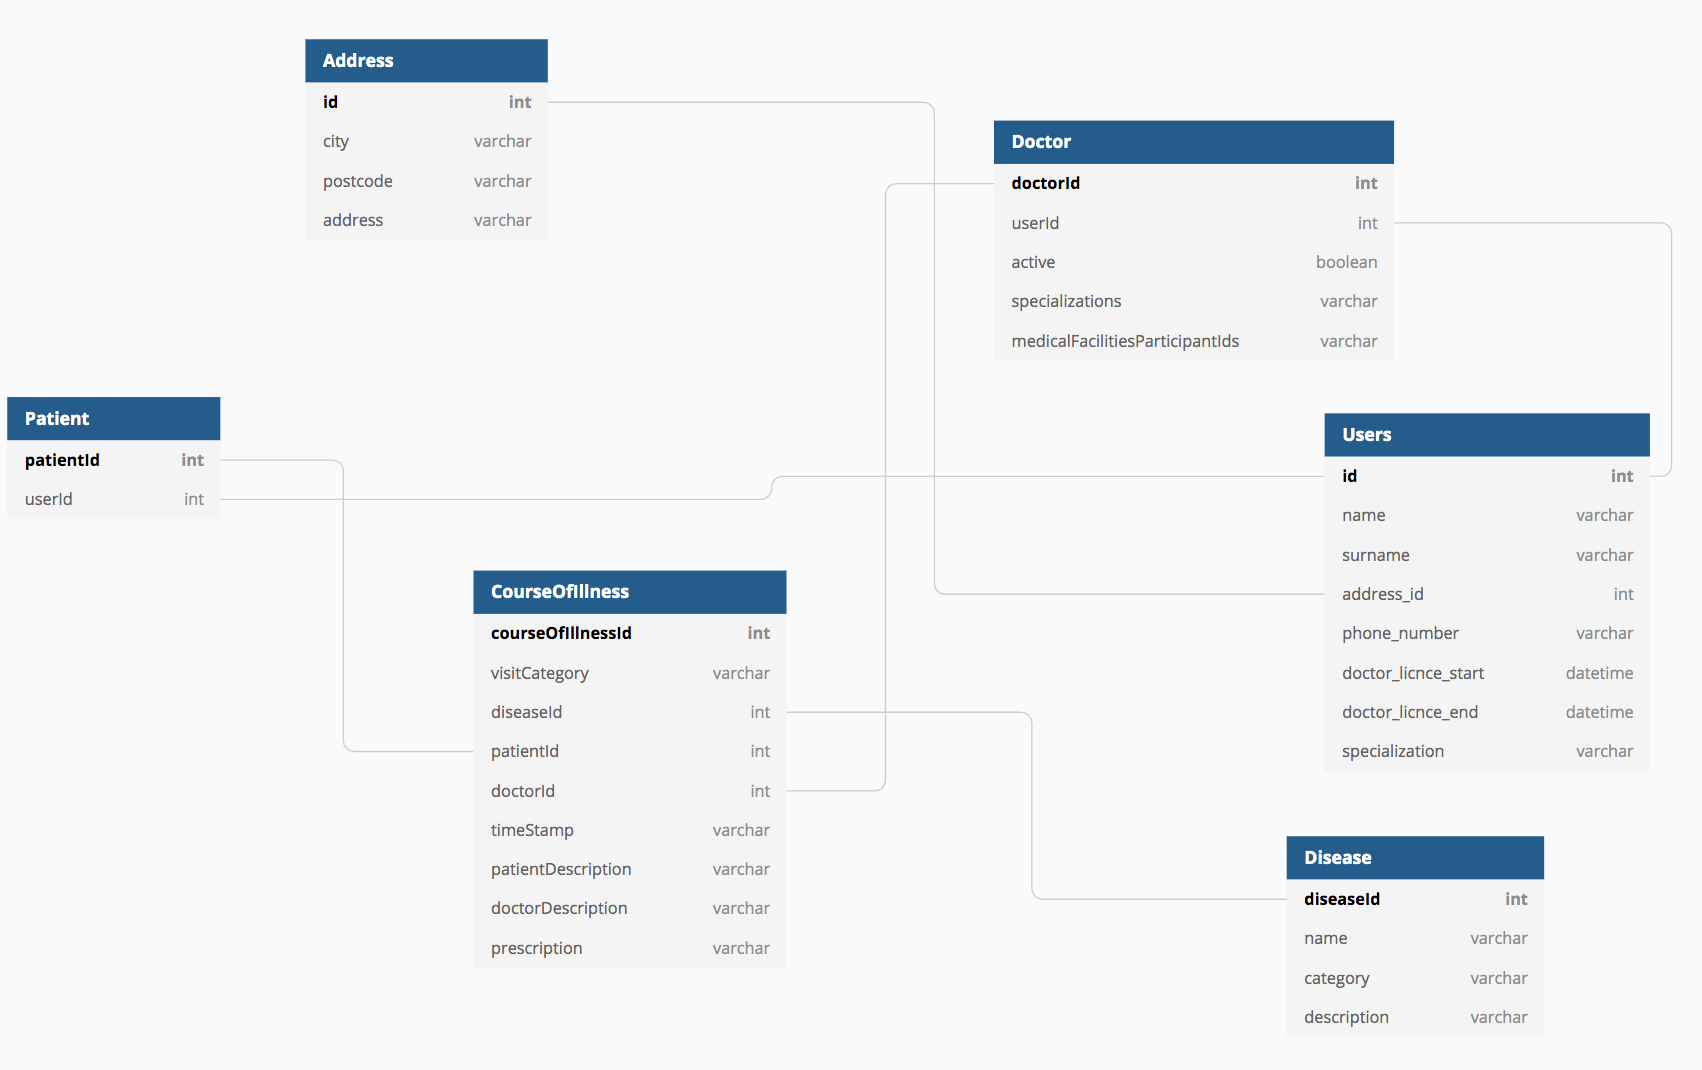
\includegraphics[width=15cm]{pictures/diagram}
\caption{Diagram ER bazy danych}
\end{figure}

\subsection{Aplikacja - backend}
\subsubsection{Endpointy}
Dzięki ogromnej popularności aplikacji internetowych opartych na języku \textit{Java} oraz \textit{framework Spring} możliwe było szybkie wygenerowanie dokumentacji \textit{Open API}. Pod \href{https://trunk-kartapacjentaservice.herokuapp.com/swagger-ui.html} {linkiem} dostępny jest spis wszystkich dostępnych w serwisie endpointów. Wejście w ten link będzie wymagało podania loginu i hasła (dostępnego tutaj: \ref{credentials}).

\subsubsection{Dlaczego REST?}
Zalety REST API:
\begin{itemize}
    \item Bezstanowość klienta - serwer nie ma potrzeby zapamiętywania wcześniejszego statnu, ponieważ zapytania HTTP zawierają wszystkie potrzebne informacje,
    \item Łatwość manipulowania obiektami z poziomu URL,
    \item Czytelność wykonywanych działań ze względu na Endpointy,
    \item Szybsze przetwarzanie informacji zwrotnej - uzycie JSON.
\end{itemize}

\subsubsection{Zabezpieczenie danych - API}
Większość \textit{endpointów} dostępnych w serwisie zapezpieczone jest przy użyciu metody \textit{Basic Auth}. Bez podania loginu i hasła niemożliwy jest dostęp do serwisu. Jedyne dostępne bez konieczności autoryzacji endpointy to te dotyczące logowania i rejestracji.

\subsubsection{Zabezpieczenie danych - baza danych}


\subsubsection{Ograniczenia}
\subsubsection{Możliwości dotyczące rozwoju - przyspieszenie}
\subsubsection{Rola serwera CRUD w aplikacji}

\subsection{Aplikacja - frontend}
\subsubsection{Działanie warstwy wizualnej}
\subsubsection{Prostota implementacji i wieloplatformowość}
\subsubsection{Rola warstwy wizualnej aplikcji}


\subsection{Testy obciążeniowe}
\subsubsection{Testowane zagadnienia}
\subsubsection{Wielowątkowość}
\subsubsection{Szybkość działania aplikacji}
\subsubsection{Rola testów w rozwoju aplikacji}



\nocite{craigspring}
\nocite{sql}
\nocite{algorytmy}
\nocite{springporadnik}
\nocite{springsecurity}
\nocite{rest}
\nocite{angular}

\bibliographystyle{unsrtnat}
\bibliography{references}

\end{document}

% PUNKTORY
% \begin{itemize}
% \item Public Documents
% \item All Documents
% \item Create Document
% \end{itemize}

% obrazek
% \begin{figure}[H]
% \centering
% \includegraphics[width=15cm]{pictures/deszyf_mycbc.png}
% \caption{Wykres zależności czasu deszyfrowania [ms] od wielkości pliku [MB] z uwzględnieniem własnej implementacji szyfru CBC}
% \label{pictures/szyfrowanie.png}
% \end{figure}